% ncse_new/p1_SystemsOfEquations/ch3_IterativeMethodsNonLinear/ex_JuliaSet.tex
% solutions:       ex_JuliaSet_20_1000.pdf        julia_set.m

\begin{problem}[Julia set]

\href{http://en.wikipedia.org/wiki/Julia_set}{Julia sets} are famous fractal
shapes in the complex plane.  They are constructed from the basins of attraction
of zeros of complex functions when the Newton method is applied to find them.
%In this problem we aim to visualize a Julia set.

In the space $\bbC$ of complex numbers the equation
\begin{equation}\label{eq:root_of_1} z^3=1 \end{equation}
has three solutions: $z_{1}=1$,
$z_{2}=-\frac{1}{2}+\frac{1}{2}\sqrt{3}i$,
$z_{3}=-\frac{1}{2}-\frac{1}{2}\sqrt{3}i$ (the cubic roots of unity).


\begin{subproblem}[2] \label{subprb:JuliaSet_1}
As you know from the analysis course, the complex plane $\bbC$ can be identified
with $\bbR^{2}$ via $(x,y)\mapsto z=x+iy$. Using this identification, convert
equation (\ref{eq:root_of_1}) into a system of equations $\VF(x,y) = \Vzero$ for a
suitable function $\VF:\bbR^{2}\mapsto\bbR^{2}$.

\begin{solution}
We have $$z^3 - 1 =(x+iy)^3 -1 = x^3+3ix^2y-3xy^2-iy^3-1 = x^3-3xy^2-1+i(3x^2y-y^3)=0.$$
Thus, equation \eqref{eq:root_of_1} is equivalent to
$\quad \mathbf{F}(x,y)=\left(\begin{array}{c}x^3-3xy^2-1 \\ 3x^2y-y^3\end{array}\right)=\left(\begin{array}{c}0\\0\end{array}\right).$
\end{solution}
\end{subproblem}

\begin{subproblem}[3] \label{subprb:JuliaSet_2}
Formulate the Newton iteration \lref{eq:Newton} for the non-linear equation $\VF(\Vx) =\Vzero$ with $\Vx = (x,y)^{T}$ and $\VF$ from the previous sub-problem.

\begin{solution}
The iteration of Newton's method for multiple variables reads
$$\mathbf{x}^{(k+1)} = \mathbf{x}^{(k)}-\big(D\mathbf{F}(\mathbf{x}^{(k)})\big)^{-1}\mathbf{F}(\mathbf{x}^{(k)}),$$
where $D\mathbf{F}$ is the Jacobian
$D\mathbf{F}(\mathbf{x})=\left(\begin{array}{cc} 3x^2-3y^2&-6xy\\ 6xy&3x^2-3y^2 \end{array}\right)$.
\end{solution}
\end{subproblem}

\begin{subproblem}[4] \label{subprb:JuliaSet_3}
Denote by $\Vx^{(k)}$ the iterates produced by the Newton method from the previous sub-problem with some initial vector $\Vx^{(0)}\in\bbR^{2}$.
Depending on $\Vx^{(0)}$, the sequence $\Vx^{(k)}$ will either diverge or converge to one of the three cubic roots of unity.

    Analyze the behavior of the Newton iterates using the following procedure:
    \begin{itemize}
    \item use equally spaced points on the domain $[-2,2]^2\subset\bbR^2$ as starting points of the Newton iterations,
    \item color the starting points differently depending on which of the three roots is the limit of the sequence $\Vx^{(k)}$.
 %         For instance you can create a RGB colormap .......... (a fourth color for diverging sequences).
    \end{itemize}

    \hint: useful \Matlab commands: \texttt{pcolor}, \texttt{colormap},
    \texttt{shading}, \texttt{caxis}. You may stop the iteration once you are
    closer in distance to one of the third roots of unity than $10^{-4}$.

The three (non connected) sets of points whose iterations are converging to the different $z_i$ are called Fatou domains, their boundaries are the Julia sets.

\begin{solution}
For each starting point at most \texttt{N\_it} iterations are accomplished.
For a given starting point $\mathbf{x}^{(0)}$, as soon as the condition $|{x}^{(k)}_1+i{x}^{(k)}_2-z_i| < 10^{-4},\; i\in\{1,2,3\}$ is reached, we assign a color depending on the root $z_i$ and on the number of iterations done.
Each attractor is associated to red, green or blue; lighter colors correspond to the points with faster convergence.
The points that are not converging in \texttt{N\_it} iterations are white.
We set the color scale using the \Matlab commands \texttt{colormap} and \texttt{caxis}.

%        \begin{figure}[hbt]   \begin{center}
%        \includegraphics[width=0.6\textwidth]{ex_JuliaSet_25_1000}
%        \caption{Julia set for $z^3-1=0$ on a mesh containing $1000\times1000$ points, \texttt{N\_it}=25.}
%        \end{center} \end{figure}

    \begin{figure}[hbt]   \begin{center}
        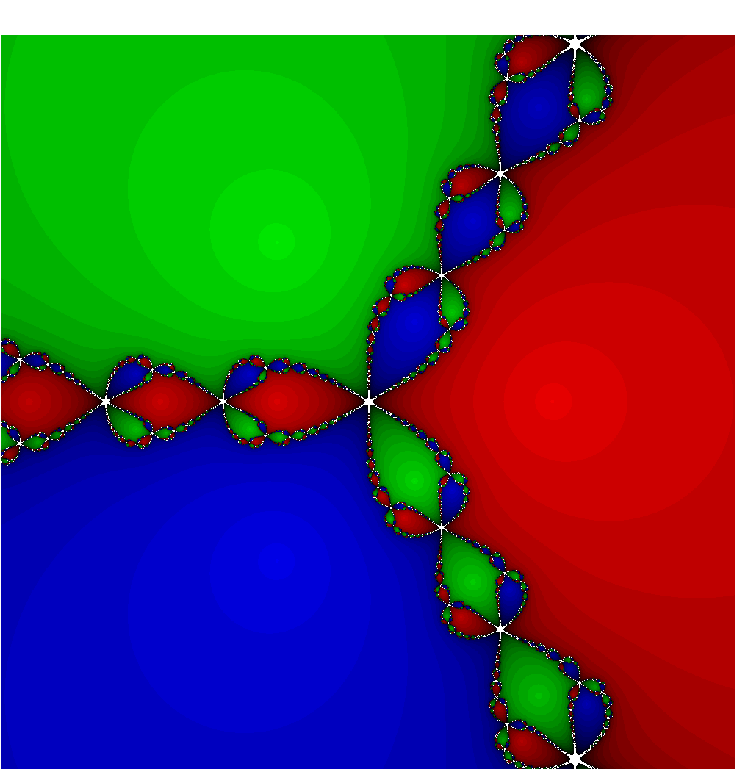
\includegraphics[width=0.6\textwidth]{\problems/ch_iterativenonlinear/PICTURES/ex_JuliaSet_20_1000.pdf} % tille: changed to pdf for better compression
        \caption{Julia set for $z^3-1=0$ on a mesh containing $1000\times1000$ points, \texttt{N\_it}=20.}
        \end{center} \end{figure}

\lstinputlisting[caption={\texttt{julia\_set.m}}, label={mc:julia_set}]
{\problems/ch_iterativenonlinear/MATLAB/julia_set.m}
\end{solution}
\end{subproblem}
\end{problem}
